%!TEX program = xelatex
% not lualatex because of a pgf bug: https://sourceforge.net/p/pgf/bugs/384/
\documentclass[12pt, a4paper]{report}
\usepackage[T1]{fontenc}
\usepackage[french]{babel}
\usepackage{hyperref}
\usepackage{utbmcovers}
\usepackage{hyphenat}
\usepackage[scale=0.75]{geometry}
\usepackage{overpic}
\usepackage{tikz}
\usepackage{float}

\usetikzlibrary{arrows, positioning}

%----------------------------------------
% hyperref configuration
%----------------------------------------

\hypersetup{
    colorlinks=true,
    urlcolor=,
}

\graphicspath{{images/}}

\newcommand\tab[1][1cm]{\hspace*{#1}}
\newcommand\TODO[1]{\textcolor{red}{TODO\@: #1}}

%----------------------------------------
% utbmcovers configuration
%----------------------------------------

\setutbmfrontillustration{versusmind.png}
\setutbmtitle{Développement d’une plateforme de recueil de consentements RGPD}
\setutbmsubtitle{Rapport de stage ST50 \hyp{} A2019}
\setutbmstudent{Nicolas BALLET}
\setutbmstudentdepartment{Département Génie Informatique}
\setutbmstudentpathway{Filière libre}
\setutbmcompany{Entreprise Versusmind}
\setutbmcompanyaddress{30 avenue du Rhin\\ 67000 Strasbourg}
\setutbmcompanywebsite{\href{versusmind.eu}{versusmind.eu}}
\setutbmcompanytutor{Philippe Didiergeorges}
\setutbmschooltutor{Vincent Hilaire}
\setutbmkeywords{Versusmind \hyp{} RGPD \hyp{} Consentement \hyp{} Signature numérique \hyp{} Cloud Microsoft Azure \newline Méthodologie Scrum \hyp{} Azure DevOps \hyp{} Angular \hyp{} Spring Boot \hyp{} Azure Functions}
\setutbmabstract{J'ai pu, durant mon stage de fin d'études à Versusmind (Strasbourg), participer au développement d'un plateforme de recueil de consentement hébergée dans le cloud Microsoft Azure.\newline L'équipe dont j'ai fait partie, utilise la methode agile Scrum. J'ai aidé à terminer une refonte graphique, mais aussi, à faire face à des problèmatiques de montée en charge et d'optimisation. Le tout sur une base de tests d'intégrations à l'aide d'Azure DevOps.}

%----------------------------------------
% document
%----------------------------------------

\begin{document}
\makeutbmfrontcover{}
    Je tiens tout d'abord à remercier Versusmind et l'UTBM pour m'avoir donné l'opportunité d'effectuer ce stage.\newline\newline
    Philippe Didiergeorges pour m'avoir suivi et guidé durant mon stage.\newline\newline
    Rémi Benoit et Jacques Lorentz pour m'avoir aidé et épaulé au sein de l'équipe durant ma formation.\newline\newline
    Francois Simond et Ahmed Zahri, qui ne faisaient pas partie de mon équipe et qui m'ont tout de même apportés un grand support.
\newpage
\tableofcontents
\chapter{Introduction}
    \section{Entreprise}
        \tab{} Versusmind est un cabinet d'architecture numérique, il est découpée en plusieurs agences, Nancy (centre), Metz, Strasbourg, Paris, Luxembourg.\newline
        Il compte aujourd'hui environ 200 employés. Il fournit aux entreprises une expertise ainsi que la réalisation leurs projets.
    \section{Projet}
        \subsection{Contexte}
            \tab{} Adopté par l’Union Européenne en avril 2016, la date d’entrée en vigueur du RGPD est le 25 mai 2018. Celui-ci oblige les entreprises à identifier les données personnelles en leur possession ainsi que leurs modalités de traitement et de protection et a pour objectifs de\@:
            \begin{enumerate}
                \item Uniformiser la réglementation au niveau européen
                \item Responsabiliser les entreprises
                \item Renforcer les droits des personnes
            \end{enumerate}
            \tab{} Le non-respect du RGPD peut mener à des sanctions financières importantes ainsi qu'a des sanctions administratives ayant un fort impact sur le fonctionnement de l'entreprise.
            Il est donc important pour les entreprises d'être en conformité avec le RGPD.\newline
            Mais migrer son système d'information pouvant coûter cher, Versusmind propose une solution nommée Central Consent Manager.
        \subsection{Central Consent Manager (CCM)}
            \tab{} CCM est système de gestion des consentements centralisé. Il va permettre aux entreprises de se libérer d'un poids en s'assurant que ses utilisateurs ont bien consentis à l'utilisation de leurs données personnelles en centralisant l'enregistrement et la vérification d'authenticité des consentements.
            \begin{figure}[H]
                \begin{center}
                    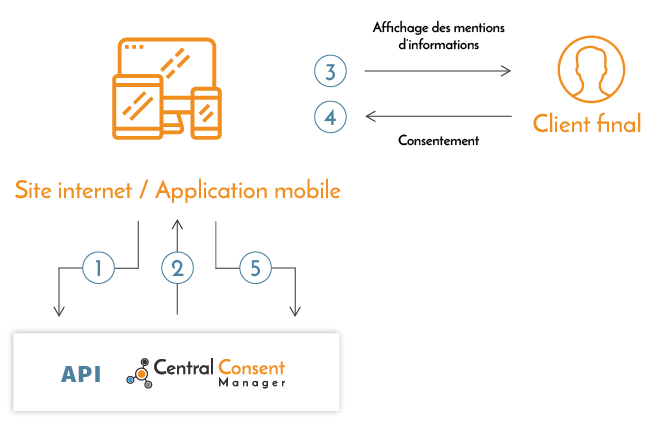
\includegraphics[width=0.8\textwidth]{ccm.png}
                \end{center}
                \caption{Fonctionnement simplifié de l'application CCM}
            \end{figure}
            \begin{enumerate}
                \item Requête sur le service de mentions pour un traitement
                \item Envoi des mentions d'informations
                \item Demande de consentement (sous forme d'e-mail ou autre)
                \item Confirmation
                \item Enregistrement du consentement
            \end{enumerate}
        \subsection{Ma mission}
            \tab{} Dans une équipe de développeurs qui évolue beaucoup, mon rôle a été d'aider au développement de la plateforme CCM, à sa mise en production et à améliorer ses performances.
\chapter{Développement}
    \section{Méthodologie Scrum}
        J'ai été intégré durant mon stage à une équipe utilisant la méthodologie Scrum, qui fait partie des méthodes de gestion de projet agiles. Cela vise à supprimer ou au moins à réduire l'effet tunnel d'une méthode de gestion classique par exemple le Cycle en V.\newline
        Le développement est découpé en cycles (de trois semaines dans le cas présent) que l'on appelle ``Sprint``.\newline
        Les Sprints sont regroupés en saisons afin de représenter un objectif général.
        Par exemple, quand j'ai démarré mon stage, le but de la saison en cours était de terminer la refonte graphique.
        Au lieu d'un cahier des charges donné au début du projet, on va le découper en User Stories tout au long du projet avec l'aide du client.\newline
        Cela permet de rester concentré sur les aspects importants et de ne pas développer de fonctionnalités qui ne seront jamais utilisées.\newline
        Un Scrum Master est assigné au projet, son rôle est d'aider l'équipe à bien suivre un fonctionnement agile ainsi qu'a s'organiser. Il est aussi là pour guider le client dans la rédaction des User Stories.
        \begin{figure}[H]
            \begin{center}
                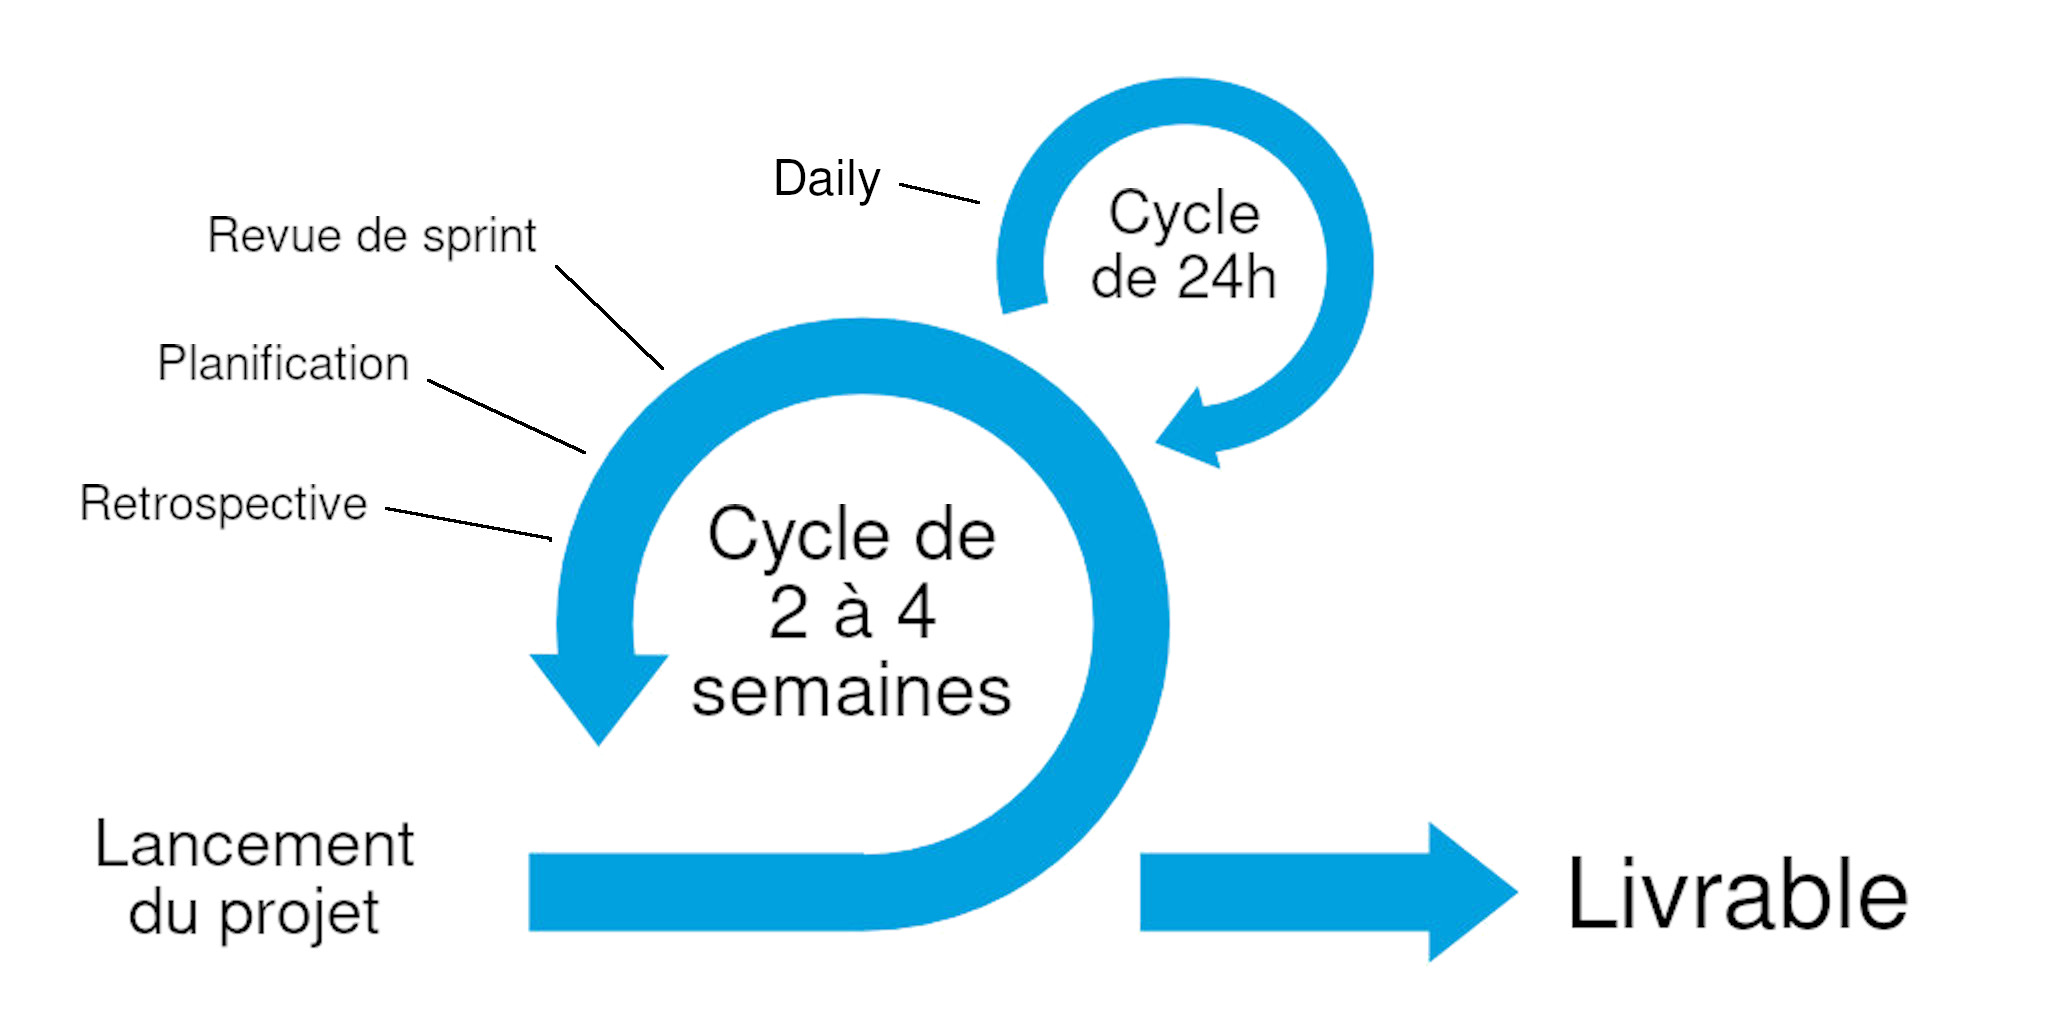
\includegraphics[width=0.9\textwidth]{scrum.jpg}
            \end{center}
            \caption{Cycle de développement Scrum}
        \end{figure}
        \subsection{Réunions journalières (Daily)}
            Chaque matin nous avons une petite réunion qui ne doit pas dépasser 15min afin d'informer rapidement le reste de l'équipe de l'avancement des différentes taches, de discuter brièvement des différents problèmes rencontrés mais aussi de choisir ensemble la priorité des différentes taches qu'il reste à faire.\newline
            Cela permet de toujours rester conscient de l'état du projet et d'avoir une vision d'ensemble du travail accompli et du travail restant.
        \subsection{Réunions inter-Sprints}
            Entre chaque Sprint, une série de réunions nous permet de rester dans la bonne direction concernant le développement du projet.
            \subsubsection{Revue de Sprint}
                Le but de la revue de Sprint est de montrer à toutes les parties prenantes (Project Owner, Scrum Master, développeurs) l'avancement du projet pendant le dernier Sprint.\newline
                L'équipe de développeurs décrit le travail accompli et après une démonstration du résultat, on discute afin de peut-être corriger la direction à prendre pour le prochain Sprint.
            \subsubsection{Planification}
                S'en suit la planification, elle se fait avec le Scrum Master ainsi que les développeurs.\newline
                On va y sélectionner les User Stories à implémenter durant le prochain Sprint. Cela constituera ce qu'on appelle ``L'objectif de Sprint``.\newline
                Sous forme d'un nombre on va se mettre d'accord sur une complexité pour chaque User Stories. Cela permet de vérifier qu'on en à bien la même compréhension. Si je propose 1 (facile) et qu'un de mes collègue propose 4 (moyen), c'est que l'un de nous deux à mal compris ce qui est attendu.\newline
                Ensuite on découpe chaque User Stories en taches concrètes et enfin on estime le temps de travail sur chaque taches.
            \subsubsection{Rétrospective}
                Et enfin, encore une fois avec le Scrum Master ainsi que les développeurs, on discute de comment s'est déroulé le dernier Sprint, des pratiques qu'on pourrait mettre en place ou améliorer, mais aussi de comment on l'a vécu et ressenti.\newline
                Cela s'inscrit dans un objectif d'amélioration de l'environnement de travail et de l'efficacité.
    \section{Architecture}
        \begin{figure}[H]
            \begin{center}
                \begin{tikzpicture}
                    % nodes
                    \node (api) at (1, 1.8) {
\includegraphics[width=0.1\textwidth]{website.png}};
                    \node [above=0 of api] {API};
                    \node (front) at (1, -1.8) {\begin{overpic}[width=0.1\textwidth]{website.png}
                        \put(60, -30){
\includegraphics[scale=.08]{ccm_logo.png}}
                    \end{overpic}};
                    \node [above=0 of front] {Front-end};
                    \node (back) at (6, 0) {
\includegraphics[width=0.1\textwidth]{server.png}};
                    \node [above=0 of back] {Back-end};
                    \node (function) at (12, 1.8) {
\includegraphics[width=0.1\textwidth]{cloud.png}};
                    \node [above=0 of function] {Azure Function};
                    \node (ejbca) at (12, -2) {
\includegraphics[width=0.2\textwidth]{ejbca.png}};

                    % arrows
                    \draw[ultra thick, ->,>=stealth] (api) -- (back);
                    \draw[ultra thick, ->,>=stealth] (front) -- (back);
                    \draw[ultra thick, double, <->,>=stealth] (back) -- node[above, sloped] {Service Bus} (function);
                    \draw[ultra thick, ->,>=stealth] (function) -- (ejbca);

                \end{tikzpicture}
            \end{center}
            \caption{Architecture globale simplifiée}
        \end{figure}
        Voici un rapide résumé des personnes destinées à utiliser l'application:
        \begin{itemize}
            \item Un administrateur Versusmind, qui pourra, via le Back-Office, accéder aux contrats souscrits avec les entreprises. Il n'a pas besoin de compétences techniques.
            \item Un administrateurs client, qui pourra, via le Back-Office, ajouter des traitements et des consentements. Il n'a pas besoin d'avoir de compétences techniques.
            \item Les développeurs clients, qui accédent à l'API du Back-end afin d'intégrer CCM dans leurs solution déjà existante.
            \item Les utilisateurs finaux, qui donneront leurs consentements au travers de la plateforme.
        \end{itemize}
        Tout d'abords je vais rapidement expliquer l'architecture du projet.
        La solution CCM est composée de différents éléments:
        \begin{itemize}
            \item Une partie Font-end écrite en HTML/CSS/Typescript avec le framework Angular, c'est le back-office d'administration, il sert les différentes pages web à l'utilisateur.
            \item Une partie Back-end écrite en Java avec le framework Spring Boot, c'est le cœur de l'application, elle peut recevoir des requêtes via le Front-end ou directement par API
            \item La gestion du chiffrement est en deux parties
                \begin{itemize}
                    \item Une instance EBJCA qui prends le rôle d'autorité de certification
                    \item Des Fonctions Azure écritent en Java qui chiffrent et vérifient les consentements. Elles communiquent avec le Back-end via des Service Bus Azure (de simples files d'attentes de messages JSON)
                \end{itemize}
            \item Une instance Redis afin de garder du cache des différentes requêtes faites à la base de données.
        \end{itemize}
        \subsection{Outils}
            Les différentes parties du stystème sont hébergées sur plateforme cloud Microsoft Azure.\newline
            On utilise aussi Azure DevOps afin d'informatiser les notions de Sprints et de User Stories mais aussi pour faciliter la gestion du code source, jouer les jeux de tests et automatiser le déploiement des nouvelles versions.
        \subsection{Front-end}
            \tab{} J'ai commencé mon stage en me formant sur l'utilisation du framework Angular sur lequel je suis maintenant à l'aise.\newline\newline
            J'ai pu ensuite aider à la fermeture d'une saison de refonte graphique en apportant mes connaissances et mon expérience en intégration web à l'équipe.\newline\newline
            J'ai aussi participé à l'amélioration et à l'enrichissement de l'interface sur toute le reste de mon stage.\newline\newline
            Aussi, tout au long de ma formation, j'ai pu faire de la veille et guider l'équipe vers une restructuration de l'architecture CSS plus maintenable et plus facile à étendre.\newline\newline
            \begin{figure}[H]
                \begin{center}
                    \fbox{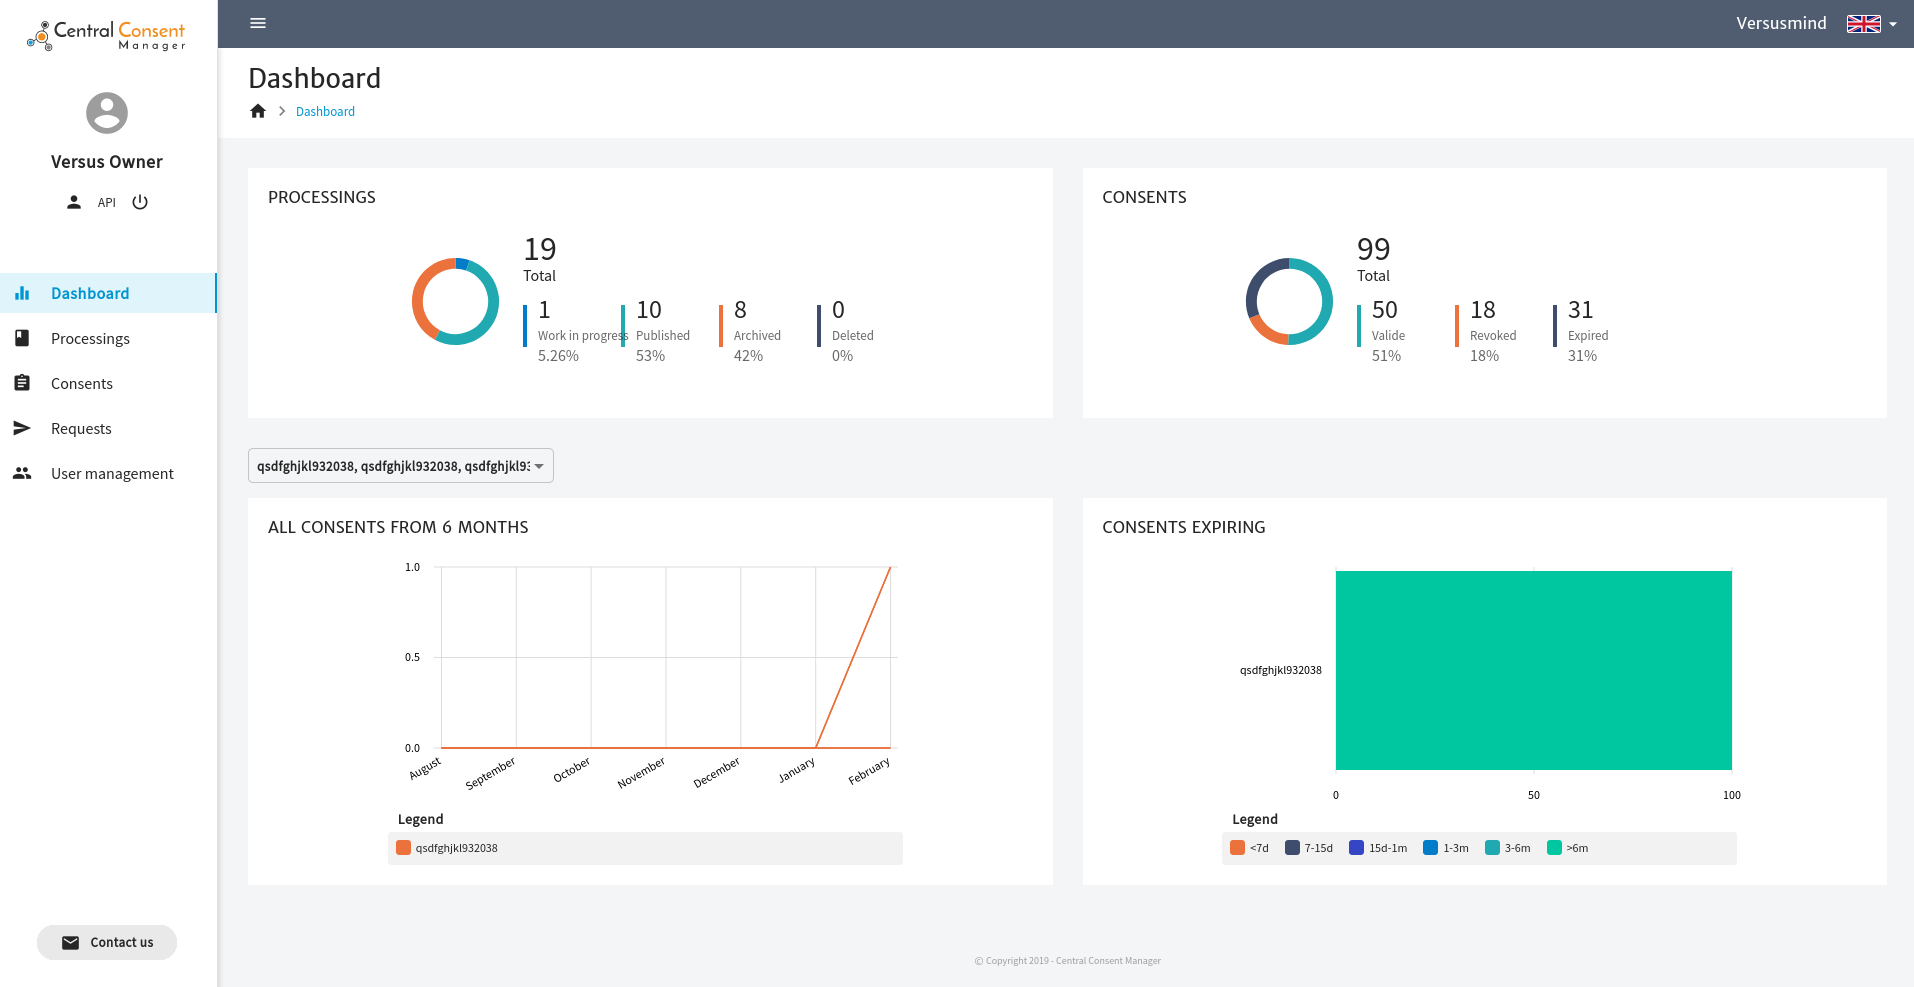
\includegraphics[width=\linewidth]{ccm_dashboard.png}}
                \end{center}
                \caption{Page d'accueil de l'application}
            \end{figure}
            \begin{figure}[H]
                \begin{center}
                    \fbox{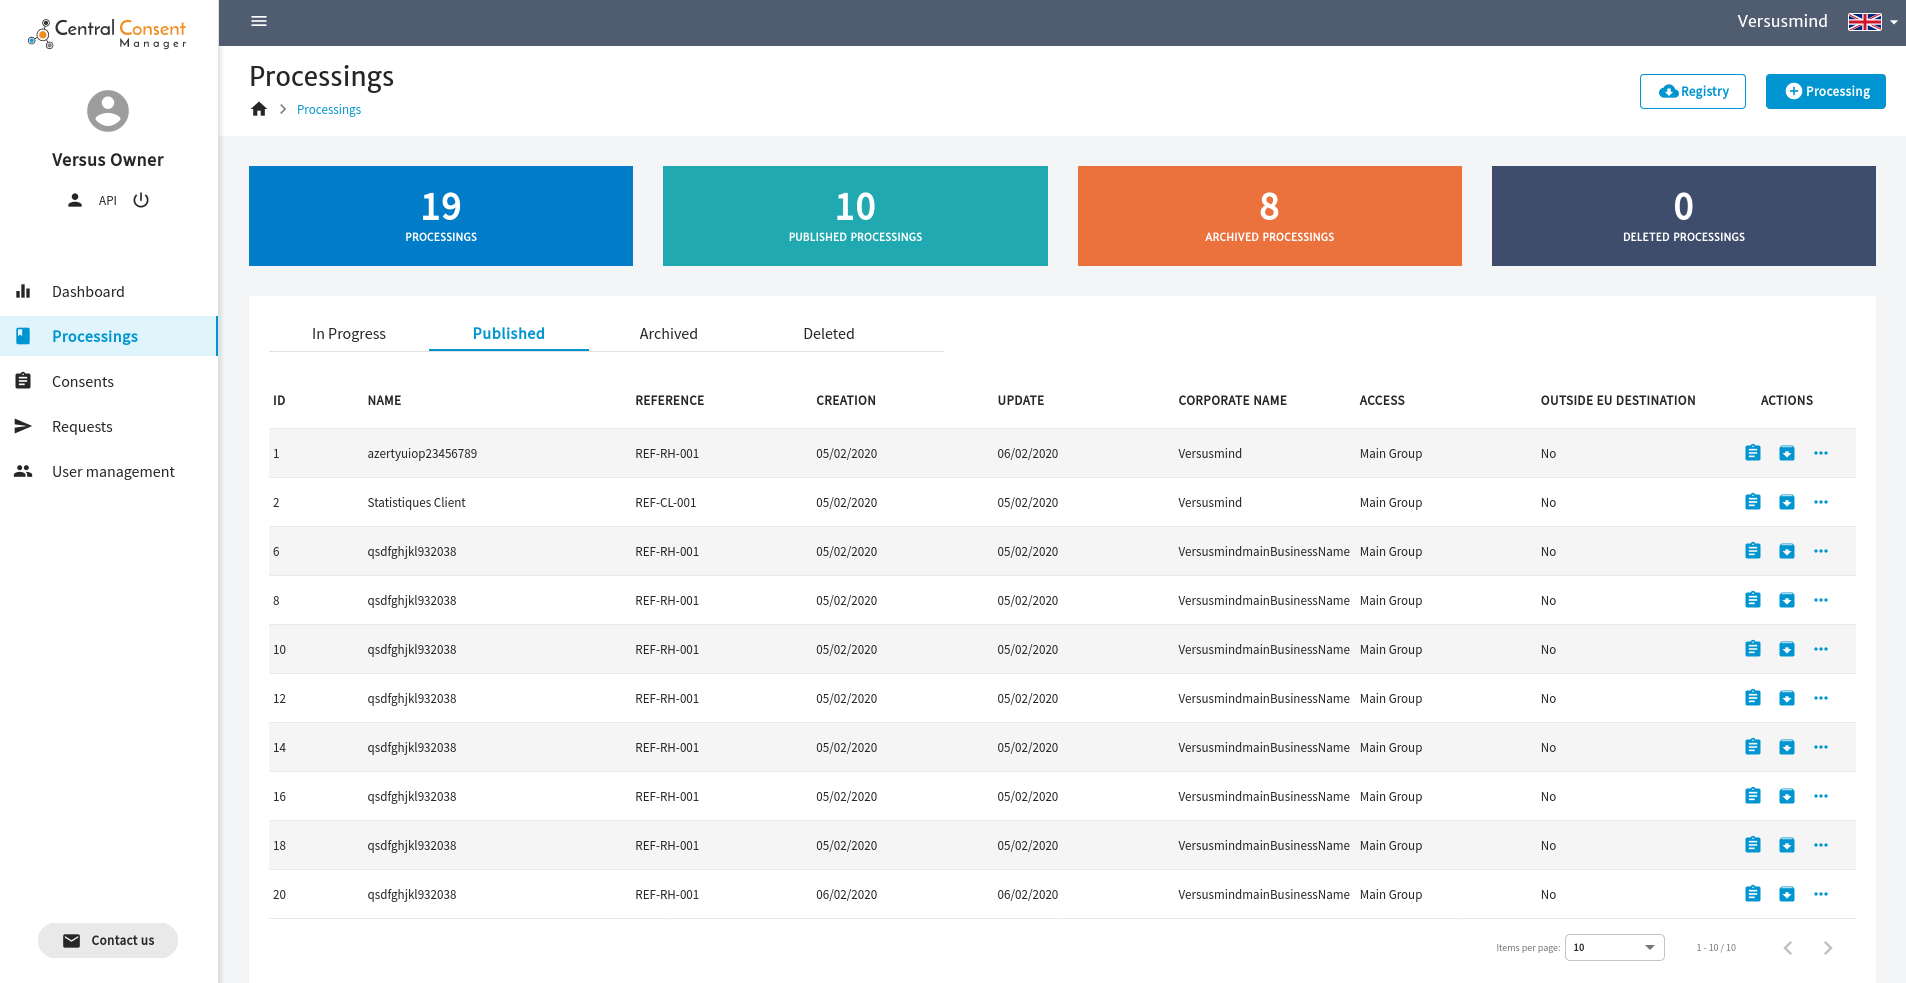
\includegraphics[width=\linewidth]{ccm_processing_list.png}}
                \end{center}
                \caption{Liste des traitements}
            \end{figure}
            \begin{figure}[H]
                \begin{center}
                    \fbox{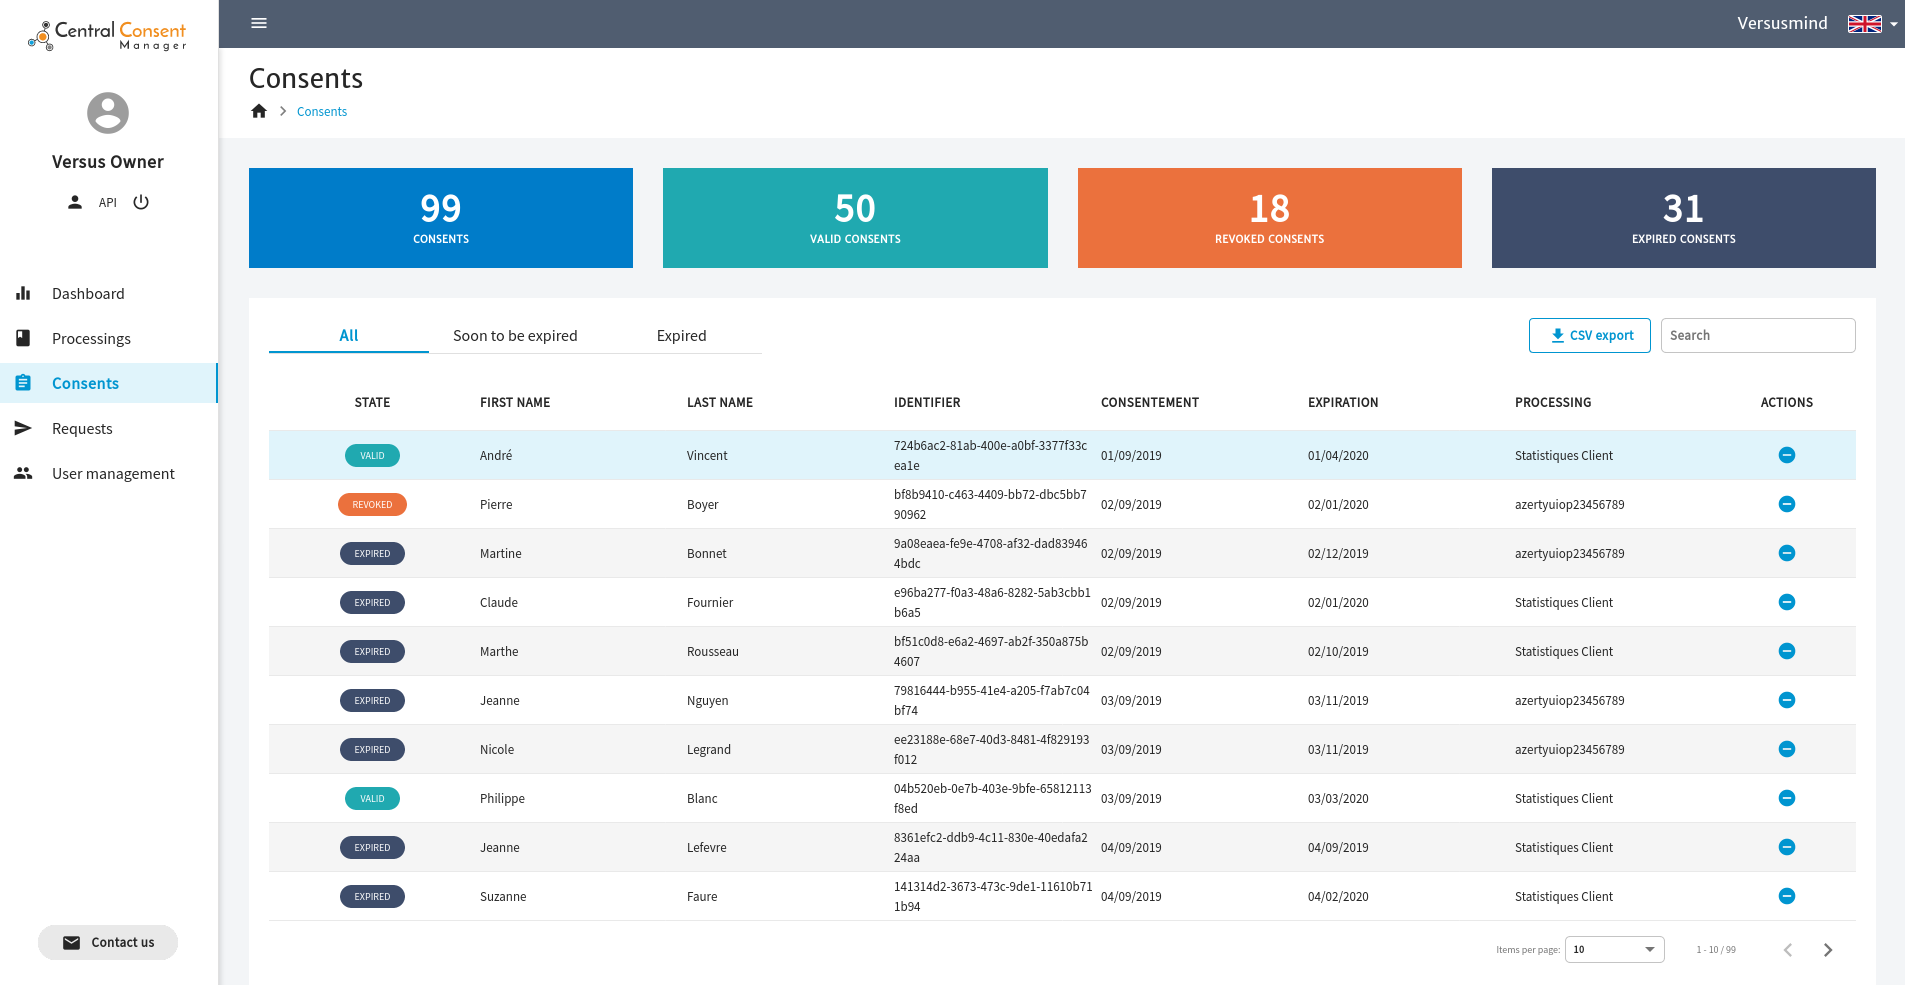
\includegraphics[width=\linewidth]{ccm_consentement_list.png}}
                \end{center}
                \caption{Liste des consentements}
            \end{figure}
            \begin{figure}[H]
                \begin{center}
                    \fbox{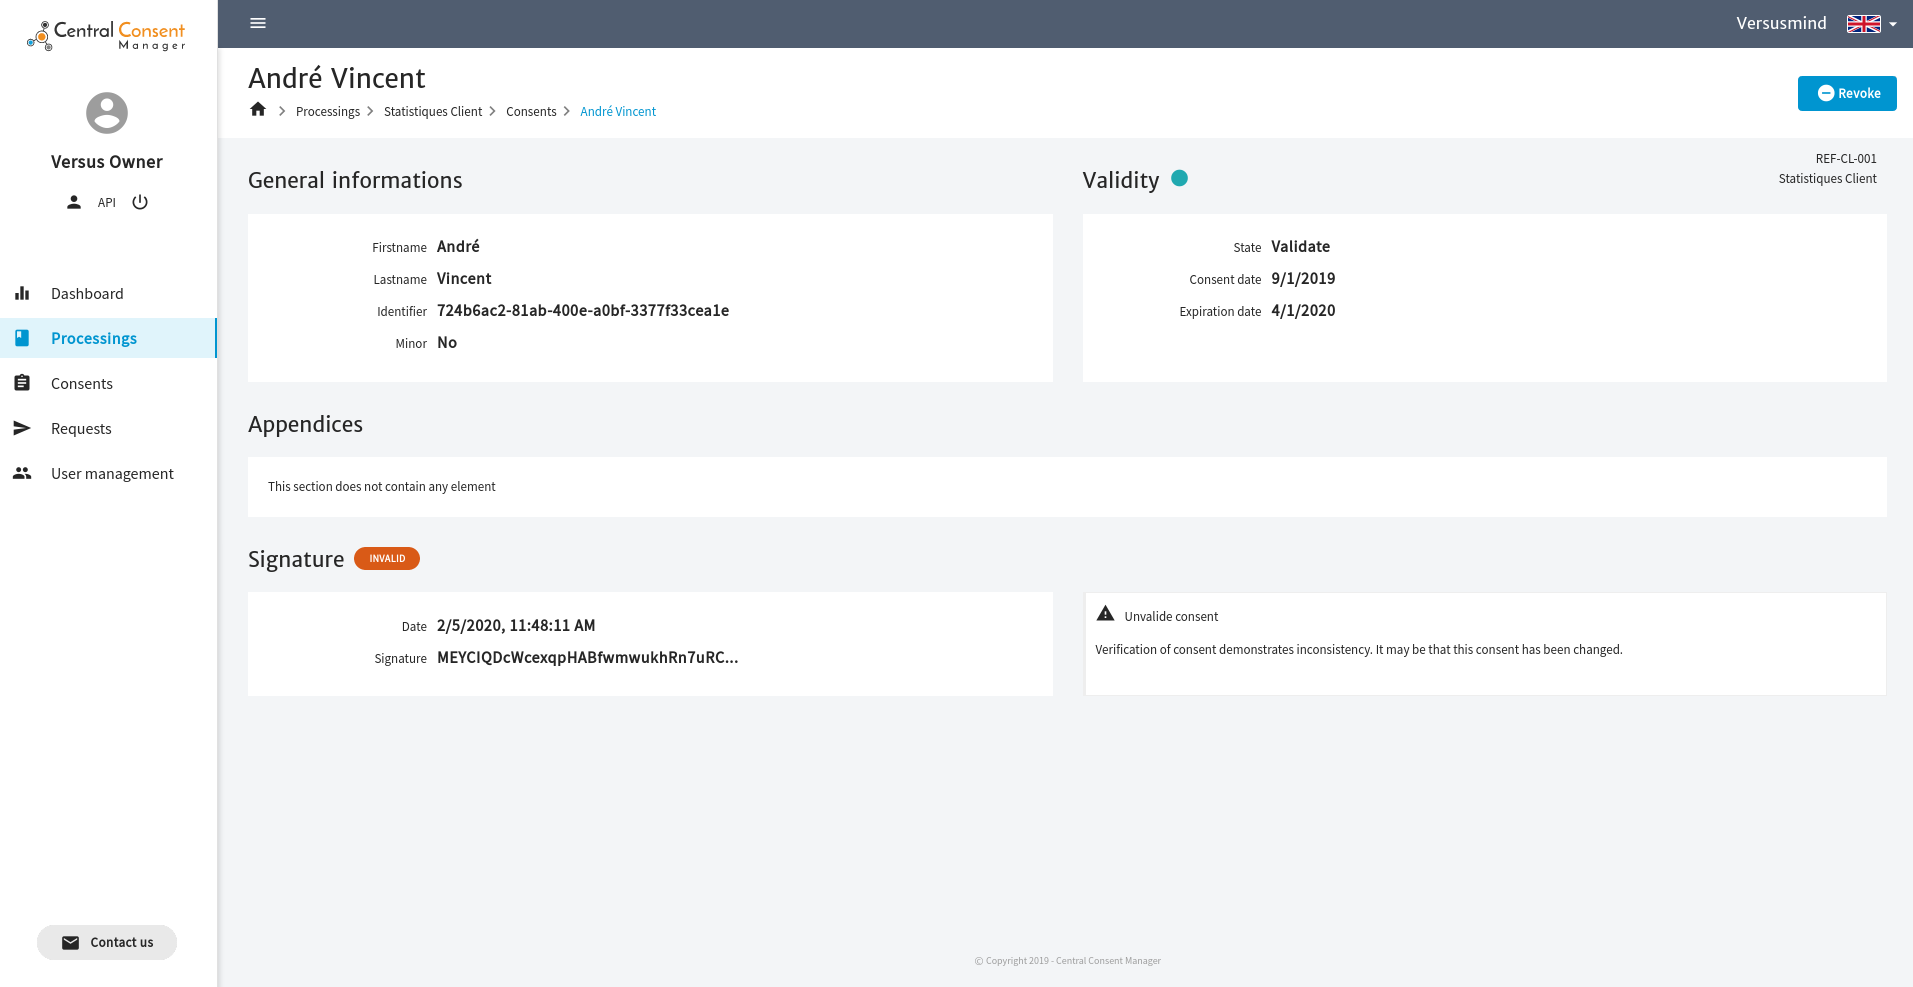
\includegraphics[width=\linewidth]{ccm_consentement_detail.png}}
                \end{center}
                \caption{Détail d'un consentement}
            \end{figure}
            \newpage
        \subsection{Back-end}
            J'ai contribué au développement du back-end du projet, sous forme d'ajout de fonctionnalités, correction de failles de sécurité, correction de bugs, etc\ldots
        \subsection{Gestion du cache}
            Je n'ai pas touché au développement de la gestion du cache côté serveur, mais j'ai participé aux discussions et aidé à la prise de décisions.
            Nous avons fait face à un problème de mise à jour des données présentes à la fois dans la base de données et dans le cache. La solution vers laquelle nous nous sommes orientés est de simplifier les requêtes faites en base pour unifier la récupération des données (abstraire le cache et la base de données) et de filtrer les données dans une couche applicative.
        \subsection{Certification numérique}
            J'ai eu à déployer une instance EJBCA assignée à l'instance de production de la plateforme CCM.\newline
            Cela comporte de la génération de clés cryptographiques, mais aussi de la manipulation de la plateforme Azure et du stockage de mots de passe sensibles car liés à la production.
        \subsection{Montée en charge}
            \tab{} Suite à la refonte graphique, nous sommes entrés dans une saison de mise en production et deux problématiques de performances sont apparues assez vite:
            \begin{itemize}
            \item Lorsqu'un nouveau client veux migrer vers CCM, une base de consentements potentiellement conséquente doit être importée.
            \item Un client doit pouvoir exporter cette base sous forme de fichier, ce qui implique une vérification de validité d'un grand nombre de consentements.
            \end{itemize}

            Suite à des tests de charge, nous avons observé qu'il faudrait environ 3 jours pour importer une base d'un million de consentements. Et plusieurs heures pour générer un export des consentements enregistrés. Ce n'était pas acceptable.\newpage
            \subsubsection{Signature}
            J'ai eu la responsabilité d'implémenter les fonctions Azure afin de paralléliser chaque création de signature numérique.
            \begin{figure}[H]
                \begin{center}
                    \begin{tikzpicture}
                        % nodes
                        \node (consentement) at (-6, 0) {
\includegraphics[width=0.1\textwidth]{file.png}};
                        \node [above=0 of consentement] {Consentement};
                        \node (function) at (0, 0) {
\includegraphics[width=0.1\textwidth]{cloud.png}};
                        \node [above=0 of function] {Azure Function};
                        \node (ejbca) at (0, -3) {
\includegraphics[width=0.2\textwidth]{ejbca.png}};
                        \node (consentement2) at (6, 0) {\begin{overpic}[width=0.1\textwidth]{file.png}
                                \put(60, -20){
\includegraphics[scale=.05]{lock.png}}
                            \end{overpic}};
                        \node [above=0 of consentement2] {Consentement signé};

                        % arrows
                        \draw[ultra thick, ->,>=stealth] (consentement) -- (function);
                        \draw[ultra thick, ->,>=stealth] (function) -- node[left] {
\includegraphics[width=0.06\textwidth]{key.png}} (ejbca);
                        \draw[ultra thick, ->,>=stealth] (function) -- (consentement2);

                    \end{tikzpicture}
                \end{center}
                \caption{Parcours de la signature d'un consentement}
            \end{figure}
            Dans la même tâche, j'ai pu implémenter la révocation de consentement en utilisant aussi des fonctions Azure.
            \subsubsection{Vérification}
            J'ai aussi eu à travailler sur la vérification des consentements et j'ai pu diviser le temps de signature par 2 tout en augmentant drastiquement le niveau de sécurité.
            \begin{figure}[H]
                \begin{center}
                    \begin{tikzpicture}
                        % nodes
                        \node (consentement) at (-6, 0) {\begin{overpic}[width=0.1\textwidth]{file.png}
                                \put(60, -20){
\includegraphics[scale=.05]{lock.png}}
                            \end{overpic}};
                        \node [above=0 of consentement] {Consentement signé};
                        \node (server) at (0, 0) {
\includegraphics[width=0.1\textwidth]{server.png}};
                        \node [above=0 of server] {Back-end (multithread)};
                        \node (ejbca) at (0, -3) {
\includegraphics[width=0.2\textwidth]{ejbca.png}};
                        \node (verified) at (7, 0) {
\includegraphics[width=0.1\textwidth]{verified.png}};
                        \node [above=0 of verified] {Validé};

                        % arrows
                        \draw[ultra thick, ->,>=stealth] (consentement) -- (server);
                        \draw[ultra thick, ->,>=stealth] (ejbca) -- node[right] {
\includegraphics[width=0.06\textwidth]{key.png}} (function);
                        \draw[ultra thick, ->,>=stealth] (server) -- (verified);

                    \end{tikzpicture}
                \end{center}
                \caption{Parcours de vérification d'un consentement non altéré}
            \end{figure}
            \begin{figure}[H]
                \begin{center}
                    \begin{tikzpicture}
                        % nodes
                        \node (ejbca) at (0, -3) {
\includegraphics[width=0.2\textwidth]{ejbca.png}};
                        \node (consentement2) at (-6, 0) {\begin{overpic}[width=0.1\textwidth]{file.png}
                                \put(60, -20){
\includegraphics[scale=.05]{lock2.png}}
                            \end{overpic}};
                        \node [above=0 of consentement2] {Consentement altéré};
                        \node (server2) at (0, 0) {
\includegraphics[width=0.1\textwidth]{server.png}};
                        \node [above=0 of server2] {Back-end (multithread)};
                        \node (error) at (6, 0) {
\includegraphics[width=0.1\textwidth]{error.png}};
                        \node [above=0 of error] {Données corrompues};

                        % arrows
                        \draw[ultra thick, ->,>=stealth] (consentement2) -- (server2);
                        \draw[ultra thick, ->,>=stealth] (ejbca) -- node[right] {
\includegraphics[width=0.06\textwidth]{key.png}} (server2);
                        \draw[ultra thick, ->,>=stealth] (server2) -- (error);

                    \end{tikzpicture}
                \end{center}
                \caption{Parcours de vérification d'un consentement altéré}
            \end{figure}
    \section{Développement dirigé par les tests (TDD)}
        Durant mon stage, j'ai appris à implémenter des tests afin de subvenir à plusieurs besoins\@:
        \begin{enumerate}
            \item Fournir une preuve de fonctionnement du code testé
            \item Prévenir d'éventuels bugs futurs
            \item S'assurer du bon fonctionnement de l'application avant son déploiement
        \end{enumerate}
        Le développement suit un cycle circulaire ou nous développons des nouvelles fonctionnalités, ce qui change le comportement de l'application, les tests ne passent donc plus. Nous réparons les test, et le cycle recommence.
        \begin{figure}[H]
            \begin{center}
                \includegraphics[width=0.5\linewidth]{TDD.jpg}
            \end{center}
            \caption{Cycle de tests et de développement}
        \end{figure}
        Pour cela, on défini le comportement unitaire de chaque composant, ainsi qu'un ou plusieurs parcours d'utilisation critiques utilisant les éléments clés de l'application.\newline
        J'ai eu l'occasion de créer différents types de tests\@:
        \begin{description}
            \item [Les tests unitaires] s'assurent que chaque composant de l'application rempli son rôle.
            \item [Les tests d'intégrations] vérifient un fonctionnement comportant plusieurs composants.
            \item [Les test de bout en bout] implémentent des User Stories completes, utilisant toutes les couches de l'application.
        \end{description}
        Et dans une démarche d'intégration continue j'ai participé à la mise en place de systèmes de tests et de déploiement automatisés sur la plateforme Azure DevOps.\newline
        J'ai pu utiliser les solutions SonarQube pour le Back-end et Eslint pour le Front-end qui s'occupent d'analyser le dépôt de code source afin d'y trouver des problèmes de sécurité, des bugs, des mauvaises pratiques ainsi que de la duplication de code.\newline
        Cela contribue à rendre le code plus stable et plus maintenable.\newline
\chapter{Conclusion}
    Ce stage m'a beaucoup apporté, d'un point de vue technique mais aussi au niveau organisationnel.\newline
    C'est pour moi une première expérience professionnelle suivant une méthode agile et j'en suis satisfait.
    Les réunions régulières m'ont permises de prendre du recul sur le travail effectué, et le travail en équipe agile à créé une dynamique dans laquelle nous nous poussions mutuellement vers le haut.\newline
    J'y ai appris à suivre un processus de développement plus stable, grâce au développement dirigé par les tests ainsi qu'a l'intégration continue via Azure DevOps.\newline
    J'ai aussi appris à développer des tests de charge et à interpréter leurs résultats afin d'en tirer des directions à prendre.\newline
    En définitive, même si le développement web n'est pas mon domaine favori, j'ai vécu une belle expérience durant ce stage et j'ai la chance de pouvoir rester au près de Versusmind et de peut-être approfondir des sujets qui me tiennent plus à cœur.
\appendix
\chapter{Personas}
    Les différents rôles dans l'application:
    \subsubsection{Versusmind}
        La société éditrice du logiciel
    \subsubsection{Propriétaire}
        La personne physique représentant le Responsable de traitement (Directeur général/Président par exemple) et ayant la capacité d'engager l'organisme.
    \subsubsection{Admin client}
        Par exemple: Un RSSI et/ou un Délégué à la protection des données (DPO) qui doivent pouvoir avoir tous les droits de lecture/écriture ainsi qu'un droit de gestion des Utilisateurs / Consultant.\newline
        Le RSSI et le DPO gèrent conjointement le projet de mise en conformité au RGPD au sein d'un organisme.\newline
        Si aucun des deux acteurs n'est nommé au sein d'un organisme et n'a pas vocation à être nommé, il est recommandé de désigner un "Référent données personnelles" ayant en charge le projet de mise en conformité.
    \newpage
    \subsubsection{Utilisateurs}
        Par exemple : Le directeur/directrice du service communication de l'organisme qui souhaite créer une newsletter en lien avec les clients de l'organisme ou des prospects ayant consenti sur le site internet de l'organisme.\newline
        Cette newsletter nécessite le consentement des clients et doit apparaître au registre des traitements.\newline
        Le directeur/directrice du service communication complète donc la partie correspondante dans le registre après que le RSSI et/ou le DPO ou, à défaut, le "Référent données personnelles" lui a octroyé les droits.
    \subsubsection{Consultant}
        Un consultant est une personne qui n'a que des droits de lecture sur le registre ou le consentement.\newline
        Par exemple: Une personne du service communication qui doit suivre les consentement sans avoir besoin de les modifier.\newline
        Ou encore: Une stagiaire qui a besoin d'y accéder pour travailler mais n'a pas soit la responsabilité nécessaire, soit le besoin de bénéficier d'un droit d'écriture.\newline
\makeutbmbackcover{}
\end{document}
